\chapter{Discussão}

\par
Analisando os resultados das tabelas, podemos observar que os melhores desempenhos foram do modelo Autorregressivo (AR) e a rede neural CNN. Os maiores lucros observados foram de ambos os modelos, com AR fechandouma carteira com +27\% de lucro, e o CNN com a carteira com +11\% de lucro, ambos com o investimento inicial de R\$ 100.000,00.

\begin{figure}[hbt]
\centering
\caption{\label{figure:figura1}Diferentes métricas, na média, para os modelos testados, bem como acurácia das operações com lucro (primeira métrica).}
  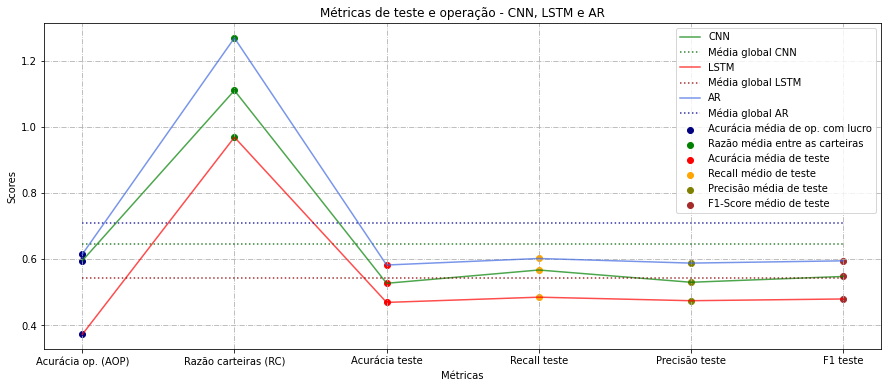
\includegraphics[scale=0.5]{figures/img1.png}
  Fonte: O autor do relatório.
\end{figure}

\par
O AR é um modelo robusto utilizado em previsões em séries temporais, então seu ótimo desempenho foi esperado. Já o modelo LSTM, para os parâmetros aqui testados, não apresentou bons resultados, principalmente se comparado ao CNN. É notável que o LSTM teve as métricas numéricas muito mais precisas que ambos AR e CNN; isso significa que o modelo teve boa capacidade de aproximar o valor previsto do fechamento para o valor real de fechamento, que se ilustra no gráfico de operação do LSTM pela proximidade entre o real e o previsto. Apesar dos valores aproximados, entretanto, as medidas das saídas categóricas ficaram inferiores, tanto no F1-Score quanto na acurácia geral, exemplificando um lucro baixo (ou prejuízo), visto que o lucro é diretamente proporcional aos movimentos classificados corretamente o maior número de vezes possível.

\par
O modelo AR apresentou média global maior que o CNN, mas suas acurácias médias de operações com lucro foram próximas, respectivamente 61\% e 59\%. Apesar das diferenças entre as acurácias no teste dos modelos (AR com 58\% e CNN com 52\%), o lucro final está diretamente relacionado com a porcentagem de operações com lucro, que em ambos os casos estão próximas de 60\%.

\par
A figura abaixo compara as funções densidade de probabilidade entre os valores obtidos nos experimentos de teste e \textit{trading} para o modelo CNN, respectivamente utilizando as métricas de acurácia da previsão dos movimentos e a acurácia de lucro nas operações realizadas.

\begin{figure}[hbt]
\centering
\caption{\label{figure:figura1}Distribuição das acurácias para os experimentos realizados com o CNN, em todos os períodos, bem como as distribuições para as operações que utilizaram as previsões do CNN, para todos os resultados em todos os períodos.}
  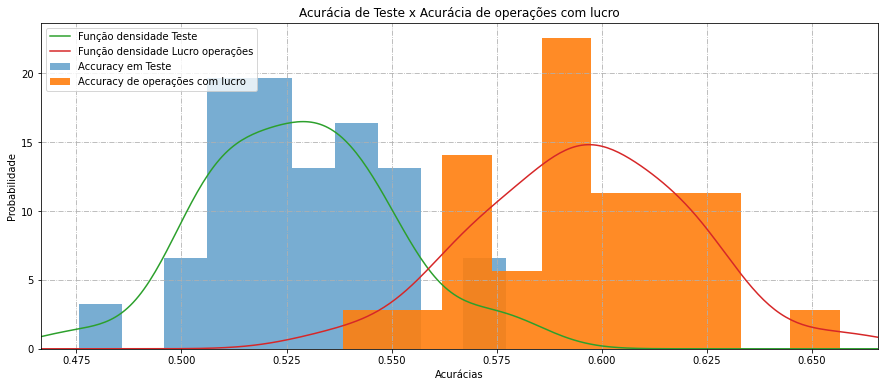
\includegraphics[scale=0.5]{figures/img14.png}
  Fonte: O autor do relatório.
\end{figure}

\par
Podemos notar que, para valores de acurácia em teste que tendem a 0.6, a acurácia de operações com lucro atinge, nessa posição, seu ponto médio. É possível traçar um paralelo entre a acurácia de teste e a acurácia de operação, levantando a hipótese de que existe uma relação diretamente proporcional entre as duas variáveis; esta hipótese também explicaria o porquê do modelo LSTM ter um desempenho ineficiente em operação, contrastando com sua precisão em termos numéricos (R2 e MSE), visto que a proximidade do valor previsto com o real não implica em acertar o movimento das ações; podemos, por exemplo, prever um valor abaixo – ainda que próximo – de uma ação, e equivocadamente classifica-la em “baixa”.

\par
Comparando as métricas de teste e acurácia de acerto em operação do CNN com o Modelo \textit{Naive} (Figura 4.6.1), observamos a maior diferença na acurácia das operações com lucro, que salta de 34\% para 59\% (+73\% de acurácia de acerto). É interessante notar que esse aumento possibilitou uma carteira final aproximadamente +38\% acima do Modelo \textit{Naive}, que na realidade finalizou com uma carteira em 80\% do valor inicial (apresentou prejuízo). Também fica evidente a diferença quando comparamos o ganho médio (em R\$), para as operações com lucro, no qual o CNN apresenta aproximadamente +988\% de lucro.

\par
Comparando o desempenho em operação do CNN com o \textit{Naive} Trading, a acurácia média de operações com lucro foi de +20\% para o CNN, com lucro médio das operações com lucro saltando de R\$ 4,21 para R\$ 192,77. O lucro final das carteiras aqui salta de R\$ 104,99 para R\$ 11.145,49 com o CNN.

\par
O desempenho do CNN frente às técnicas ingênuas, tanto para o modelo \textit{Naive} utilizando Classifications Trading quanto para o \textit{Naive} \textit{Trading} (operando sem modelo), se demonstrou mais eficiente e lucrativo. Entretanto, comparativamente ao modelo AR, seu desempenho em todos os casos foi inferior. Comparativamente, a média das diferenças entre as carteiras finais foi de R\$ 11.145,49 para o CNN, bem como R\$ 27.029,99 para o AR. É interessante notar que as acurácias de lucro por operações são semelhantes (aproximadamente 60\%); para as acurácias máximas observadas durante os experimentos, o CNN teve a AOL atingindo 65\% de operações com lucro, em contrapartida de 63\% para o modelo AR.

\par
Se compararmos o desempenho dos modelos com o algoritmo \textit{Real Movements Trading}, podemos estabelecer um parâmetro de desempenho ótimo, do qual acerta todas as operações, e então avaliar cada técnica individualmente. O RMT fez 64 operações, das quais acertou todas, na média entre os anos 2019 e 2020. Para o CNN, temos 52\% de acerto das operações considerando um desempenho perfeito; no caso do AR temos 63\%; LSTM com 30\%; Modelo \textit{Naive} com 34\%. É notável que o CNN e o AR tiveram desempenhos muito superiores às demais técnicas, e para as métricas, de forma geral, um desempenho próximo de 60\% implica também em 60\% de aproveitamento em relação ao desempenho perfeito.


\par
Considerando como ideal o algoritmo RMT, bem como as métricas do modelo AR todas ótimas, os modelos foram avaliados segundo os critérios abaixo:


%---------------TABLE
\begin{table}[H]
\footnotesize
\centering
\caption{Critérios para avalair os modelos segundo suas métricas.}
\begin{tabular}{ccccc|cll}
\cline{1-6}
0.65 & $\geq$ & \textit{accuracy} & $\geq$ & 0.60 & \textit{ótimo} &  &  \\
0.60 & > & \textit{accuracy} & $\geq$ & 0.55 & \textit{bom} &  &  \\
0.55 & > & \textit{accuracy} & $\geq$ & 0.50 & \textit{razoável} &  &  \\
0.50 & > & \textit{accuracy} & $\geq$ & 0.00 & \textit{ruim} &  &  \\
1.00 & $\geq$ & R2 & $\geq$ & 0.90 & \textit{ótimo} &  &  \\
0.90 & > & R2 & $\geq$ & 0.70 & \textit{bom} &  &  \\
0.70 & > & R2 & $\geq$ & 0.00 & \textit{ruim} &  &  \\
1.00 & $\geq$ & AOL & $\geq$ & 0.55 & \textit{ótimo} &  &  \\
0.55 & > & AOL & $\geq$ & 0.50 & \textit{bom} &  &  \\
0.50 & > & AOL & $\geq$ & 0.00 & \textit{ruim} &  &  \\ \cline{1-6}
\end{tabular}
\center{Fonte: Autor do relatório. Dados das tabelas 8, 9 e 11.}
\end{table}


\par
Para os experimentos realizados neste trabalho, observamos que:

\begin{itemize}
    
    \item{A \textit{rede CNN} apresentou um desempenho \textbf{bom} na classificação dos movimentos}
    \item{A \textit{rede CNN} apresentou um desempenho \textbf{razoável} nas previsões numéricas}
    \item{A \textit{rede CNN} apresentou um desempenho \textbf{ótimo} para AOL em \textit{trading}}
    \item{A \textit{rede LSTM} apresentou um desempenho \textbf{ruim} nas classificações dos movimentos}
    \item{A \textit{rede LSTM} apresentou um desempenho \textbf{ruim} para AOL em \textit{trading}}
    \item{A \textit{rede LSTM} apresentou um desempenho \textbf{bom} nas previsões numéricas}
    \item{O \textit{modelo AR} apresentou um desempenho \textbf{ótimo} na classificação dos movimentos}
    \item{O \textit{modelo AR} apresentou um desempenho \textbf{ótimo} nas previsões numéricas}
    \item{O \textit{modelo AR} apresentou um desempenho \textbf{ótimo} para AOL em \textit{trading}}
    \item{O \textit{modelo Naive} apresentou um desempenho \textbf{ruim} na classificação dos movimentos}
    \item{O \textit{modelo Naive} apresentou um desempenho \textbf{bom} nas previsões numéricas}
    \item{O \textit{modelo Naive} apresentou um desempenho \textbf{ruim} para AOL em \textit{trading}}
\end{itemize}